\UseRawInputEncoding
\documentclass[12pt]{article}
\title{ECE 102 Homework 2}
\usepackage{subcaption}
\author{Lawrence Liu}
\usepackage{graphicx}
\usepackage{amsmath}
\setlength{\parskip}{\baselineskip}%
\setlength{\parindent}{0pt}%
\usepackage{listings}
\begin{document}
\maketitle
\section*{Problem 1}
\subsection*{(a)}
\begin{align*}
h(t)&=\int_{-\infty}^{t-1}e^t\cos(2\tau+2-2t)\delta(\tau)e^{2-\tau}d\tau\\
&=\int_{-\infty}^{t-1}e^t\cos(2-2t)\delta(\tau)e^{2}d\tau\\
&=e^{t+2}\cos(2-2t)u(t-1)
\end{align*}
Since $h(t,\tau)=h(t-\tau)=0$ for $t<\tau$, this system is causal. Furthermore, since $e^t$ is not bounded (it goes to $\infty$ as $t\to\infty$), this system is not BIBO stable.
\subsection*{(b)}
\begin{align*}
h(t)&=e^{-t}\int_{-\infty}^{t}e^\tau[\cos(t)\cos(\tau)-\sin(t)\sin(\tau)]\delta(\tau)d\tau\\
&=e^{-t}\int_{-\infty}^{t}e^\tau\cos(t+\tau)\delta(\tau)d\tau\\
&=e^{-t}\int_{-\infty}^{t}\cos(t)\delta(\tau)d\tau\\
&=e^{-t}\cos(t)u(t)
\end{align*}
Since $h(t,\tau)=h(t-\tau)=0$ for $t<\tau$, this system is causal. To find if the system is BIBO stable, let us input a bounded signal $|x(t)|<M<+\infty$ and determine if the output is bounded as well
$$
|y(t)|=\left|e^{-t}\int_{-\infty}^{t}e^\tau[\cos(t)\cos(\tau)-\sin(t)\sin(\tau)]x(\tau)d\tau\right|
$$
Since $e^t$ and $e^-t$ are positive for any $t$ we get
\begin{align*}
|y(t)|&=e^{-t}\int_{-\infty}^{t}e^\tau|\cos(t+\tau)x(\tau)|d\tau\\
&=e^{-t}\int_{-\infty}^{t}e^\tau|\cos(t+\tau)||x(\tau)|d\tau\\
&\leq e^{-t}\int_{-\infty}^{t}e^\tau|\cos(t+\tau)|Md\tau\\
&\leq Me^{-t}\int_{-\infty}^{t}e^\tau d\tau\\
&=Me^{-t}e^t\\
&=M<+\infty
\end{align*}
Thus this system is BIBO stable.
\subsection*{(c)}
\begin{align*}
h(t)&=\int_{-\infty}^{t-1}e^{-(t-\tau)}\delta(\tau-2)d\tau\\
&=\int_{-\infty}^{t-1}e^{-(t-2)}\delta(\tau-2)d\tau\\
&=e^{2-t}u(t-3)
\end{align*}
Since $h(t,\tau)=h(t-\tau)=0$ for $t<\tau$, this system is causal.
To find if the system is BIBO stable, let us input a bounded signal $|x(t)|<M<+\infty$ and determine if the output is bounded as well
\begin{align*}
|y(t)|&=\left|\int_{-\infty}^{t-1}e^{-(t-\tau)}x(\tau-2)d\tau\right|\\
&=\int_{-\infty}^{t-1}e^{-(t-\tau)}|x(\tau-2)|d\tau\\
&\leq M\int_{-\infty}^{t-1}e^{-(t-\tau)}d\tau\\
&=M e^{(t-1)-t}=Me^{-1}<+\infty
\end{align*}
Thus this system is BIBO stable.
\section*{Problem 2}
\subsection*{(a)}
\begin{align*}
h_1(t,\tau)&=\delta(t-\tau)u(t)-\int_{-\infty}^{t-2}e^{-(t-\sigma)}\delta(\sigma-\tau)u(\sigma)d\sigma\\
&=\delta(t-\tau)u(\tau)-\int_{-\infty}^{t-2}e^{-(t-\tau)}\delta(\sigma-\tau)u(\tau)d\sigma\\
&=\delta(t-\tau)u(\tau)-e^{-(t-\tau)}u(\tau)\int_{-\infty}^{t-2}\delta(\sigma-\tau)d\sigma\\
&=\boxed{\delta(t-\tau)u(\tau)-e^{-(t-\tau)}u(\tau)u(t-2-\tau)}
\end{align*}
\begin{align*}
h_2(t,\tau)&=\int_{-\infty}^{t}\delta(\sigma-\tau)u(\sigma)d\sigma\\
&=\int_{-\infty}^{t}\delta(\sigma-\tau)u(\tau)d\sigma\\
&=\boxed{u(\tau)u(t-\tau)}
\end{align*}
\subsection*{(b)}
Since these systems as cascading we have
\begin{align*}
h_{12}(t,\tau)&=\int_{-\infty}^{\infty}h_1(\sigma,\tau)h_2(t,\sigma)d\sigma\\
&=\int_{-\infty}^{\infty}\left(\delta(\sigma-\tau)u(\tau)-e^{-(\sigma-\tau)}u(\tau)u(\sigma-2-\tau)\right)u(\sigma)u(t-\sigma)d\sigma
\end{align*}
Since these systems are linear we can break it up into two integrals $\int_{-\infty}^{\infty}\delta(\sigma-\tau)u(\tau)u(\sigma)u(t-\sigma)d\sigma$ and $\int_{-\infty}^{\infty}e^{-(\sigma-\tau)}u(\tau)u(\sigma)u(\sigma-2-\tau)u(t-\sigma)d\sigma$. For the first integral we get
\begin{align*}
\int_{-\infty}^{\infty}\delta(\sigma-\tau)u(\tau)u(\sigma)u(t-\sigma)d\sigma&=\int_{-\infty}^{\infty}\delta(\sigma-\tau)u^2(\tau)u(t-\tau)d\sigma\\
&=u(\tau)u(t-\tau)\int_{-\infty}^{\infty}\delta(\sigma-\tau)d\sigma\\
&=u(\tau)u(t-\tau)
\end{align*}
To evaluate the second integral let us first evaluate it in two regions, when $t>\tau+2$, $\tau>0$, and everywhere else. When $t>\tau+2$ and $\tau>0$ we get
\begin{align*}
\int_{-\infty}^{\infty}e^{-(\sigma-\tau)}u(\tau)u(\sigma)u(\sigma-2-\tau)u(t-\sigma)d\sigma&=\int_{2+\tau}^{t}e^{-\sigma+\tau}d\sigma\\
&=\left.-e^{-\sigma+\tau}\right|_{\sigma=2+\tau}^{t}\\
&=e^{-2}-e^{-t+\tau}
\end{align*}
And everywhere else we get 
$$\int_{-\infty}^{\infty}e^{-(\sigma-\tau)}u(\tau)u(\sigma)u(\sigma-2-\tau)u(t-\sigma)d\sigma=0$$
Thus we get that 
$$h_{12}(t,\tau)=\boxed{u(\tau)u(t-\tau)-u(\tau)u(t-2-\tau)(e^{-2}-e^{-t+\tau})}$$
\subsection*{(c)}
To find if the system is BIBO, let us input a bounded signal $|x(t)|<M<+\infty$ and determine if the output $w(t)$ is bounded as well. To find that let us first find if $y(t)$ is stable
\begin{align*}
|y(t)|&=\left|x(t)u(t)-\int_{-\infty}^{t-2}e^{-(t-\tau)}x(\tau)u(\tau)d\tau\right|\\
&\leq\left|x(t)u(t)\right|+\left|-\int_{-\infty}^{t-2}e^{-(t-\tau)}x(\tau)u(\tau)d\tau\right|\\
&\leq Mu(t)+\left|\int_{-\infty}^{t-2}e^{-(t-\tau)}x(\tau)u(\tau)d\tau\right|\\
&\leq Mu(t)+M\left|\int_{-\infty}^{t-2}e^{-(t-\tau)}u(\tau)d\tau\right|\\
&=Mu(t)+M\left|\int_{0}^{t-2}e^{-(t-\tau)}d\tau\right|\\
&=Mu(t)+M\left|\left.e^{-(t-\tau)}\right|_{\tau=0}^{t-2}\right|\\
&=Mu(t)+M\left|e^{-2}-e^{t}\right|
\end{align*}
This is not bounded, since as $t\to\infty$, $y(t)\to\infty$ and thus $y(t)$ is not stable. If $y(t)$ is not stable then $w(t)$ is also not stable since the integral of $\infty$ from $-\infty$ to $\infty$ is also $\infty$.
\subsection*{(d)}
Since these systems as cascading we have
\begin{align*}
h_{21}(t,\tau)&=\int_{-\infty}^{\infty}h_2(\sigma,\tau)h_1(t,\sigma)d\sigma\\
&=\int_{-\infty}^{\infty}u(\sigma)u(\sigma-\tau)(\delta(t-\sigma)u(\sigma)-e^{-(t-\sigma)}u(\sigma)u(t-2-\sigma))d\sigma\\
&=\int_{-\infty}^{\infty}\delta(t-\sigma)u(\sigma)u(\sigma-\tau)d\sigma-\int_{-\infty}^{\infty}e^{-(t-\sigma)}u(\sigma)u(t-2-\sigma)u(\sigma-\tau)d\sigma\\
&=u(t)u(t-\tau)-\int_{-\infty}^{\infty}e^{-(t-\sigma)}u(\sigma)u(t-2-\sigma)u(\sigma-\tau)d\sigma
\end{align*}
$\int_{-\infty}^{\infty}e^{-(t-\sigma)}u(\sigma)u(t-2-\sigma)u(\sigma-\tau)d\sigma$ can evaluate to 3 different expression
\begin{itemize}
\item When $t<2$ or when $\tau>t-2$, $u(\sigma)u(t-2-\sigma)u(\sigma-\tau)=0$, thus we get
$$\int_{-\infty}^{\infty}e^{-(t-\sigma)}u(\sigma)u(t-2-\sigma)u(\sigma-\tau)d\sigma=0$$
\item When $t>2$ and $\tau<0$, $u(\sigma)u(t-2-\sigma)u(\sigma-\tau)=1$ for $0<\sigma<t-2$ thus we get
\begin{align*}
\int_{-\infty}^{\infty}e^{-(t-\sigma)}u(\sigma)u(t-2-\sigma)u(\sigma-\tau)d\sigma&=\int_{0}^{t-2}e^{-(t-\sigma)}d\sigma\\
&=\left.e^{\sigma-t}\right|_{\sigma=0}^{t-2}\\
&=e^{-2}-e^{-t}
\end{align*}
\item When $t>2$ and $0<\tau<t-2$ we get $u(\sigma)u(t-2-\sigma)u(\sigma-\tau)=1$ for $\tau<\sigma<t-2$ thus we get
\begin{align*}
\int_{-\infty}^{\infty}e^{-(t-\sigma)}u(\sigma)u(t-2-\sigma)u(\sigma-\tau)d\sigma&=\int_{\tau}^{t-2}e^{-(t-\sigma)}d\sigma\\
&=\left.e^{\sigma-t}\right|_{\sigma=\tau}^{t-2}\\
&=e^{-2}-e^{\tau-t}
\end{align*}
\end{itemize}

Thus we get that
$$h_{21}(t,\tau)=\boxed{\begin{cases}
0 & t<0 \text{ or } \tau>t\\
1 & 0<t<2 \text{ or } t>\tau>t-2\\
1+e^{-t}-e^{-2} & t>2 \text{ and } \tau<0\\
1+e^{\tau-t}-e^{-2} & t>2 \text{ and } 0<\tau<t-2
\end{cases}}$$
\pagebreak
\section*{Problem 3}
\subsection*{(a)}
\begin{lstlisting}
t=-5:0.01:5;
y=sin(pi*(2*t-1))./(pi*(2*t-1));

figure;
plot(t,y);
xlabel('t');
ylabel('y(2t −1)');
title('Signal y(2t −1) vs t');
\end{lstlisting}
\begin{figure}[h]
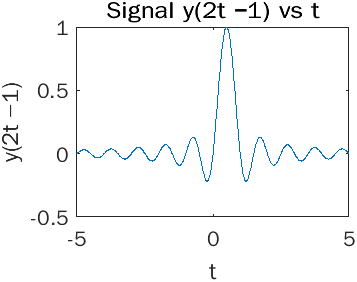
\includegraphics[width=8cm]{3a}
\end{figure}
\subsection*{(b)}
\begin{lstlisting}
t=-5:0.01:5;
y=sin(pi*t)./(pi*t);

figure;
plot(t,y.^2);
xlabel('t');
ylabel('y^2(t)');
title('Signal y^2(t) vs t');
\end{lstlisting}
\begin{figure}[h]
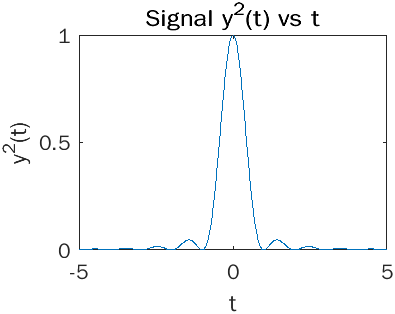
\includegraphics[width=8cm]{3b}
\end{figure}
\subsection*{(c)}
\begin{lstlisting}
t = linspace(-5, 5, 1000);
dt = t(2) - t(1);
    
y = sin(pi*t)./(pi*t);
y(51)=1;
z = conv(y,y,'same')*dt;

figure;
plot(t,z);
xlabel('t');
ylabel('z(t)');
title('Signal z(t) vs t');
\end{lstlisting}
\begin{figure}[h]
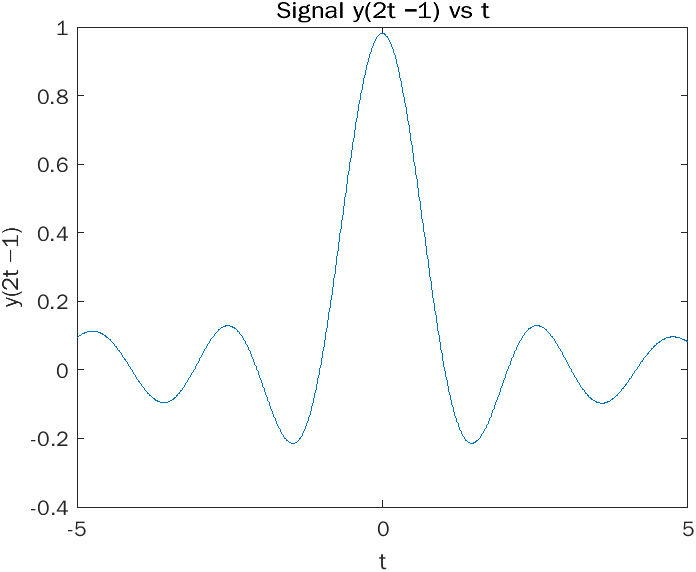
\includegraphics[width=8cm]{3c}
\end{figure}
\pagebreak
\subsection*{(d)}
\begin{lstlisting}
fy = @(t) sin(pi*t)./(pi*t);
hfig=figure;
%plot out z(2t-1)
t = linspace(-11, 11, 1000);
dt = t(2) - t(1);
y=fy(t);
%y(51)=1;
z = conv(y,y,'same')*dt;

subplot(3,1,1);
plot((t+1)/2,z);
xlim([-5,5]);
xlabel('t');
ylabel('z(2t-1)');
title('Signal z(2t-1) vs t');

%plot out {y(t)*y(2t-1)}
t = linspace(-5, 5, 1000);
dt = t(2) - t(1);
y=fy(t);
y2=fy(2*t-1);
subplot(3,1,2);
plot(t,conv(y,y2,'same')*dt);
xlabel('t');
ylabel('{y(t)*y(2t-1)}');
title('Signal {y(t)*y(2t-1)} vs t');

%plot out {y(2t-1)*y(2t-1)}
subplot(3,1,3);
plot(t,conv(y2,y2,'same')*dt);
xlabel('t');
ylabel('{y(2t-1)*y(2t-1)}');
title('Signal {y(2t-1)*y(2t-1)} vs t');
%print figure
print(hfig, '-djpeg', '3d');
\end{lstlisting}
\begin{figure}[h]
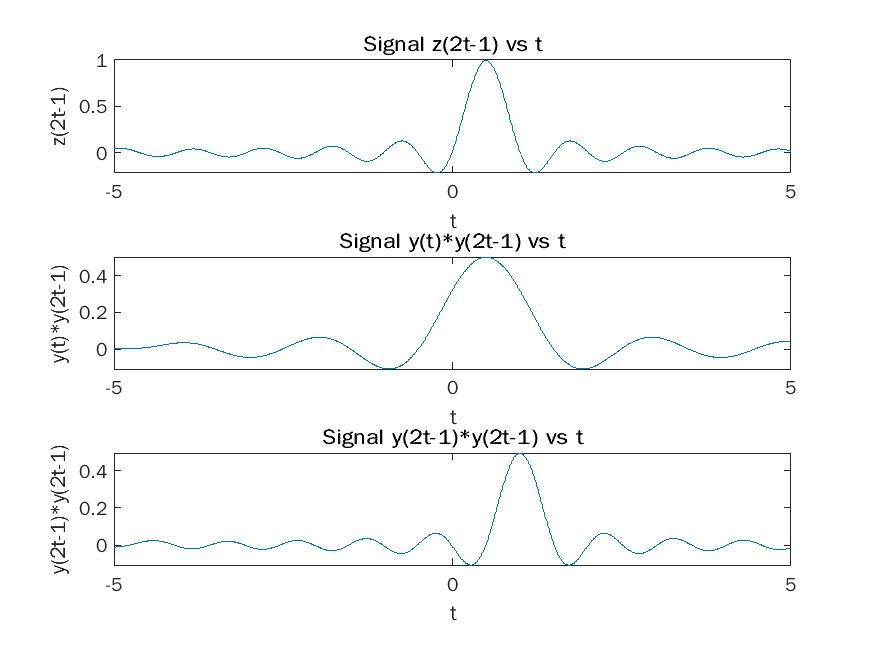
\includegraphics[width=8cm]{3d}
\end{figure}
Thus the answer neither.
\section*{Problem 4}
\subsection*{(a)}
\begin{lstlisting}
t=linspace(-3,3,1000);
%define functions
u=@(t) heaviside(t);
x = @(t) sin(2.*pi.*t).*u(t + 1).*u(-t + 1);
h=@(t) u(t)-u(t-1);

%plot x(t)
figure;
plot(t,x(t));
xlabel('t');
ylabel('x(t)');
title('Signal x(t) vs t');
%plot x(t)
figure;
plot(t,h(t));
xlabel('t');
ylabel('h(t)');
title('Signal h(t) vs t');
\end{lstlisting}
\begin{figure}[h]
\centering
\begin{subfigure}{.5\textwidth}
  \centering
  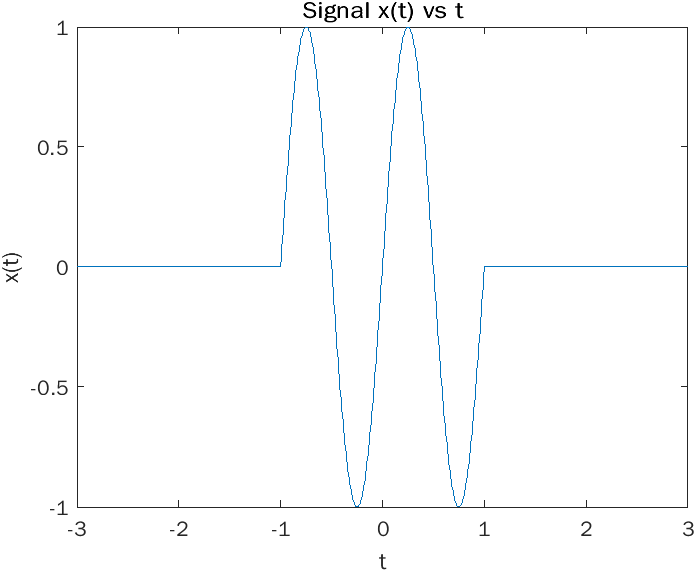
\includegraphics[width=.9\linewidth]{4a1}
\end{subfigure}%
\begin{subfigure}{.5\textwidth}
  \centering
  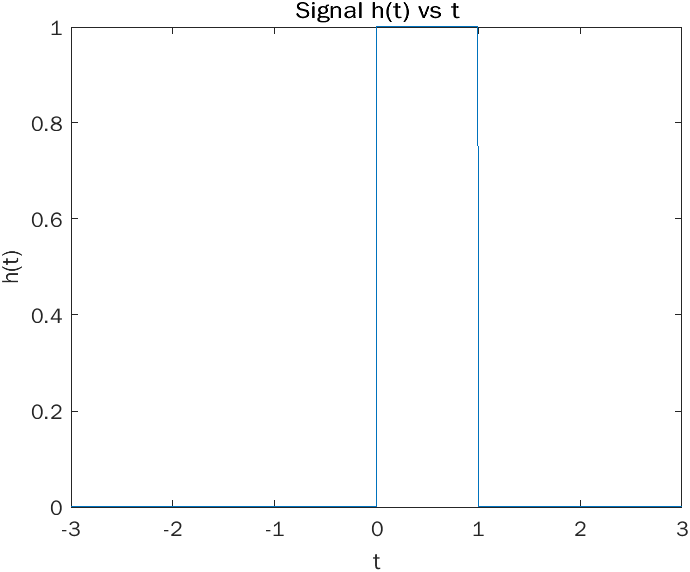
\includegraphics[width=.9\linewidth]{4a2}
\end{subfigure}
\end{figure}
\subsection*{(b)}
\begin{align*}
y_1(t)&=x(t)*h(t)\\
&=\int_{-\infty}^{\infty}x(\tau)h(t-\tau)d\tau\\
&=\int_{-\infty}^{\infty}\sin(2\pi\tau)u(\tau+1)u(-\tau+1)\left(u(t-\tau)-u(t-\tau-1)\right)d\tau
\end{align*}
Under different values of $t$, $\int_{-\infty}^{\infty}\sin(2\pi\tau)u(\tau+1)u(-\tau+1)\left(u(t-\tau)-u(t-\tau-1)\right)d\tau$ yields different expressions
\begin{itemize}
\item When $t\leq-1$ or $t\geq2$, $u(\tau+1)u(-\tau+1)\left(u(t-\tau)-u(t-\tau-1)\right)=0$ for all values of $\tau$, thus we get
$$\int_{-\infty}^{\infty}\sin(2\pi\tau)u(\tau+1)u(-\tau+1)\left(u(t-\tau)-u(t-\tau-1)\right)d\tau=0$$
\item When $-1<t<0$, $u(\tau+1)u(-\tau+1)\left(u(t-\tau)-u(t-\tau-1)\right)=1$ for $-1<\tau<t$, thus we get
\begin{align*}
\int_{-\infty}^{\infty}\sin(2\pi\tau)u(\tau+1)u(-\tau+1)\left(u(t-\tau)-u(t-\tau-1)\right)d\tau&=\int_{-1}^{t}\sin(2\pi\tau)d\tau\\
&=\left.-\frac{\cos(2\pi\tau)}{2\pi}\right|_{\tau=-1}^{t}\\
&=\frac{1-\cos(2\pi t)}{2\pi}
\end{align*}
\item When $0<t<1$ we get $u(\tau+1)u(-\tau+1)\left(u(t-\tau)-u(t-\tau-1)\right)=1$ for $t-1<\tau<t$, since the period of $\sin(2\pi\tau)$ is $1$ we get
$$\int_{-\infty}^{\infty}\sin(2\pi\tau)u(\tau+1)u(-\tau+1)\left(u(t-\tau)-u(t-\tau-1)\right)d\tau=0$$
\item When $1<t<2$ we get $u(\tau+1)u(-\tau+1)\left(u(t-\tau)-u(t-\tau-1)\right)=1$ for $t-1<\tau<1$, thus we get
\begin{align*}
\int_{-\infty}^{\infty}\sin(2\pi\tau)u(\tau+1)u(-\tau+1)\left(u(t-\tau)-u(t-\tau-1)\right)d\tau&=\int_{t-1}^{1}\sin(2\pi\tau)d\tau\\
&=\left.-\frac{\cos(2\pi\tau)}{2\pi}\right|_{\tau=t-1}^{1}\\
&=\frac{\cos(2\pi(t-1))-1}{2\pi}
\end{align*}
\end{itemize}
Therefore we get that:
$$y_1(t)=\boxed{\begin{cases}
0 & t\leq-1\\
\frac{1-\cos(2\pi t)}{2\pi} & -1<t<0\\
0 &  0\leq t\geq1\\
\frac{\cos(2\pi(t-1))-1}{2\pi} & 1<t<2\\
0 & t\geq2
\end{cases}}$$
\end{document}